\documentclass[unicode,notheorems]{beamer}

\makeatletter
\def\input@path{{styles/}}
\makeatother

\mode<presentation>
{
	\usetheme[numbers,totalnumbers,compress,nologo]{Statmod}
	\setbeamercovered{transparent}
}

\usefonttheme[onlymath]{serif}
\setbeamertemplate{navigation symbols}{}

\usepackage[utf8]{inputenc}
\usepackage[T2A]{fontenc}
\usepackage[russian]{babel}
\usepackage{amsmath,amssymb,amsthm,amsfonts}
\usepackage{graphicx}
\usepackage{float}
\usepackage{tikz}

\def\figurename{Рис.}
\setbeamertemplate{caption}[numbered]
\setbeamertemplate{caption label separator}{. }

\title{Некоторые алгоритмы для обнаружения прямых линий на изображениях}
\author{Фалин Алексей Дмитриевич, гр. 22.Б04-мм}
\institute[СПбГУ]{Санкт-Петербургский государственный университет \\
	Математико-механический факультет \\
	Кафедра статистического моделирования \\
	\vspace{0.5cm}
	Научный руководитель: д.ф.-м.н. Голяндина Н.Э.}
\date{Санкт-Петербург\\2025 г.}

\begin{document}

\begin{frame}[plain]
	\titlepage
\end{frame}

\section{Постановка задачи}

\begin{frame}{Постановка задачи}
	\begin{block}{Постановка задачи обнаружения прямых}
		\begin{itemize}
			\item Наблюдаемое изображение: матрица яркостей $\mathbf{M} \in \mathbb{R}^{m \times n}$.

			\item В рассматриваемом эксперименте компонента сигнала $\mathbf{S}$ такова, что пикселям на $k$-й прямой соответствует константа $c_k>0$, задающая её интенсивность, а вне прямых стоят нули.
			\item Модель наблюдения:
			\[
			\mathbf{M} = \mathbf{S} + \mathbf{R},
			\]
			где $(\bf{R})_{ij}\stackrel{\text{i.i.d.}}{\sim}\mathcal{N}(0,\sigma^2)$.
			\item Цель: по зашумлённому изображению выделить прямые линии и оценить их параметры.
		\end{itemize}
	\end{block}
\end{frame}

\begin{frame}{Пример зашумлённого изображения}
	\begin{figure}
		\centering
		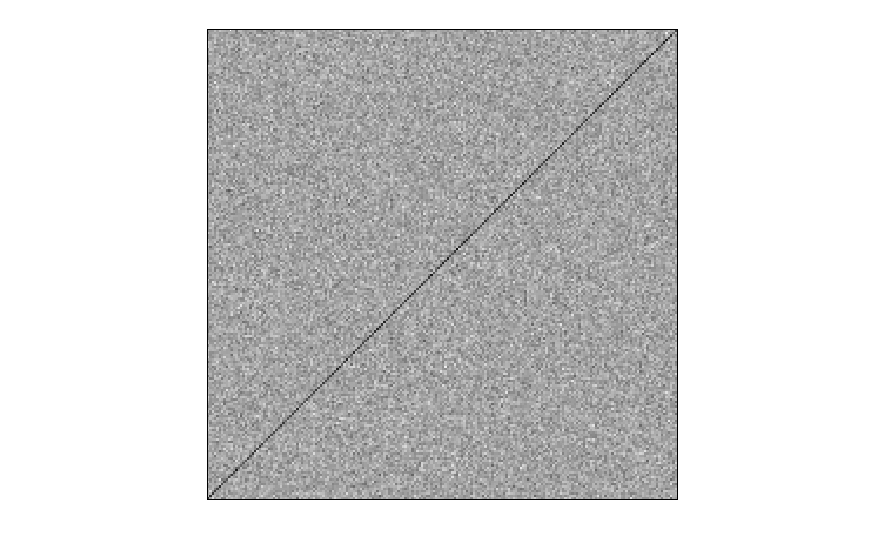
\includegraphics[width=0.7\textwidth]{images/Noisy_pic.png}
		\refstepcounter{figure}

		\vspace{0.15cm}
		{\footnotesize
		\centering
		\parbox{0.9\linewidth}{\centering \figurename~\thefigure. Зашумлённое изображение размера 100 на 100 с прямой $y=x$ и $\sigma=0.2$}
		\par}
	\end{figure}
\end{frame}

\begin{frame}{Метод Хафа и предобработка}
	\begin{itemize}
		\item Существует алгоритм Хафа, который решает задачу оценки параметров прямых на изображении.
		\item На практике преобразование Хафа обычно применяется после некоторой предобработки изображения.
		\item В этой работе метод Хафа используется как этап финальной оценки параметров после шумоподавления.
	\end{itemize}

	\vspace{0.25cm}
	\begin{block}{Почему возникает этап предобработки}
		\begin{itemize}
			\item Метод Хафа ищет максимумы в пространстве параметров.
			\item Шум порождает ложные активные точки и ложные максимумы в аккумуляторном массиве.
			\item Поэтому перед методом Хафа изображение сначала подвергают шумоподавлению.
		\end{itemize}
	\end{block}
\end{frame}

\begin{frame}{Методы шумоподавления перед методом Хафа}
	\begin{itemize}
		\item В качестве предобработки обычно используют стандартные методы шумоподавления, например \texttt{BM3D}, Медианный фильтр и Фильтр Винера.
		\item Наряду с ними можно использовать алгоритм, основанный на преобразовании Фурье и методе CSSA.
		\item В численном эксперименте рассматривается вариант \texttt{CSSA ROW-ROW}.
	\end{itemize}

	\vspace{0.25cm}
	\begin{block}{Задача работы}
		Сравнить \texttt{CSSA ROW-ROW} со стандартными методами шумоподавления по точности оценивания параметров прямой после применения метода Хафа.
	\end{block}
\end{frame}

\begin{frame}{Цель работы и план доклада}
	\begin{block}{Цель работы}
		Сравнить алгоритмы на основе \texttt{CSSA} с классическими методами шумоподавления по точности оценивания параметров прямой после применения метода Хафа.
	\end{block}

	\vspace{0.3cm}
	\textbf{План доклада:}
	\begin{enumerate}
		\item Описание метода Хафа.
		\item Описание алгоритма на основе \texttt{CSSA} и стандартных методов шумоподавления.
		\item Численное сравнение.
	\end{enumerate}
\end{frame}

\section{Преобразование Хафа}

\begin{frame}{Преобразование Хафа: замечание о параметризации прямой}
	\small
	\begin{itemize}
		\item Часто прямую на плоскости задают в виде $y = ax + b$.
		\item Для вертикальной прямой $x = c$ коэффициент наклона $a$ не является конечным.
		\item Поэтому в методе Хафа используют перепараметризацию
		\[
		\rho = x \cos \theta + y \sin \theta.
		\]
		\item Изначально можно рассматривать параметры $\rho>0$ и $\theta\in[0,2\pi)$, где $\rho$ --- расстояние от начала координат до прямой, а $\theta$ --- угол радиус-вектора.
		\item Однако пары $(\rho,\theta)$ и $(-\rho,\theta+\pi)$ задают одну и ту же прямую, поэтому удобно использовать эквивалентную параметризацию, в которой $\rho\in\mathbb{R}$, $\theta\in[0,\pi)$.
		
	\end{itemize}
\end{frame}

\begin{frame}{Преобразование Хафа: параметризация $(\rho,\theta)$}
	\begin{figure}
		\centering
		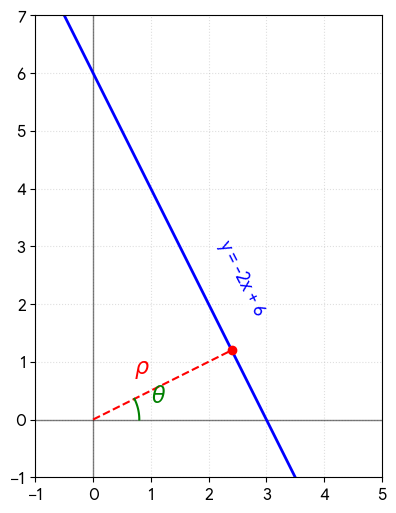
\includegraphics[width=0.5\textwidth]{images/rt_params.png}
		\caption{Параметризация прямой через $\rho$ и $\theta$}
	\end{figure}
\end{frame}

\begin{frame}{Преобразование Хафа: идея}
	\begin{itemize}
		\item После введения параметризации $(\rho,\theta)$ задачу обнаружения прямой можно перенести в пространство параметров.
		\item Для фиксированной точки изображения $(x_0,y_0)$ множество всех прямых, проходящих через неё, описывается соотношением
		\[
		\rho(\theta) = x_0 \cos \theta + y_0 \sin \theta,
		\]
		то есть одной кривой в параметрическом пространстве.
		\item Если точки $(x_1,y_1),\dots,(x_k,y_k)$ лежат на одной прямой, то соответствующие кривые проходят через общую точку $(\rho^\ast,\theta^\ast)$.
		\item Эта общая точка задаёт параметры исходной прямой.
		\item Поэтому задача выделения прямых сводится к поиску точек пересечения таких кривых, а после дискретизации --- к поиску максимумов в аккумуляторном массиве.
	\end{itemize}
\end{frame}

\begin{frame}{Аккумуляторный массив}
	\small
	\begin{block}{Определение}
		{\scriptsize
		Пусть $E$ --- множество активных точек изображения,
		$h_\rho>0$ и $h_\theta>0$ --- шаги дискретизации по параметрам $\rho$ и $\theta$.
		Сетка в пространстве параметров задаётся как
		\[
		\rho_i = -\rho_{\max} + i h_\rho,\qquad
		\theta_j = j h_\theta.
		\]
		Тогда аккумуляторный массив $A=(A_{ij})$ определяется формулой
		\[
		A_{ij} =
		\sum_{(x,y)\in E}
		\mathbf{1}\left\{
		\left| \rho_i - \bigl(x\cos\theta_j + y\sin\theta_j\bigr) \right|
		\le \frac{h_\rho}{2}
		\right\}.
		\]
		}
	\end{block}

	\begin{itemize}
		\item Параметры $h_\rho$ и $h_\theta$ задают точность дискретизации пространства параметров.
		\item Для каждой активной точки $(x,y)$ и каждого значения $\theta_j$ вычисляется $\rho = x\cos\theta_j + y\sin\theta_j$, после чего увеличивается соответствующая ячейка аккумулятора.
		\item Поэтому локальные максимумы аккумуляторного массива интерпретируются как оценки параметров прямых.
	\end{itemize}
\end{frame}

\begin{frame}{Пример аккумуляторного массива}
	\begin{figure}
		\centering
		\begin{tikzpicture}
			\node[inner sep=0] (img) {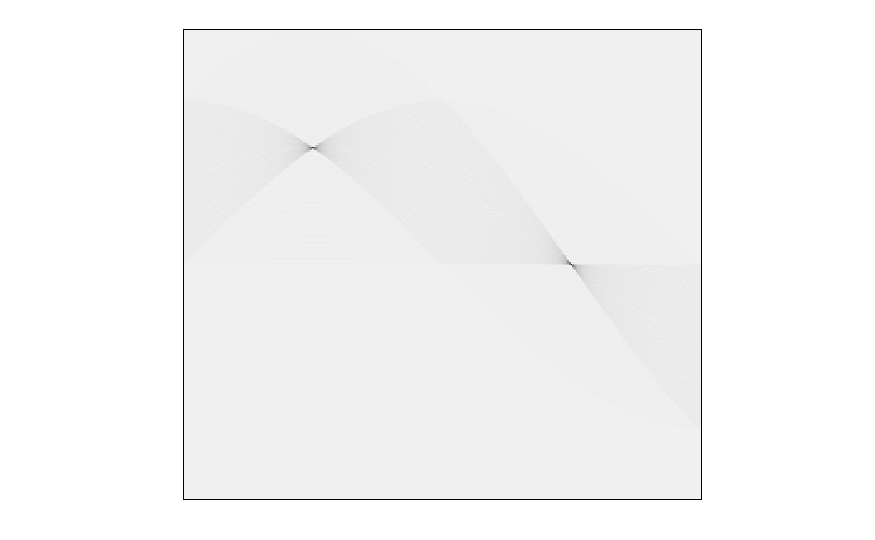
\includegraphics[width=0.82\textwidth]{images/ACCUMULATOR_pic.png}};
			\begin{scope}[blend mode=difference]
				\fill[white] (img.south west) rectangle (img.north east);
			\end{scope}
		\end{tikzpicture}
		\caption{Аккумуляторный массив для изображения с двумя прямыми}
	\end{figure}
\end{frame}

%\begin{frame}{Поиск максимумов и NMS}
%	\begin{itemize}
%		\item После заполнения аккумулятора нужно найти его локальные максимумы.
%		\item При шуме рядом с истинным максимумом часто возникает несколько близких больших значений.
%		\item Поэтому используется локальное подавление немаксимумов (NMS).
%		\item NMS оставляет только наиболее сильные пики и делает оценку параметров устойчивее.
%	\end{itemize}
%\end{frame}
%
%\begin{frame}{Аккумулятор после NMS}
%	\begin{figure}
%		\centering
%		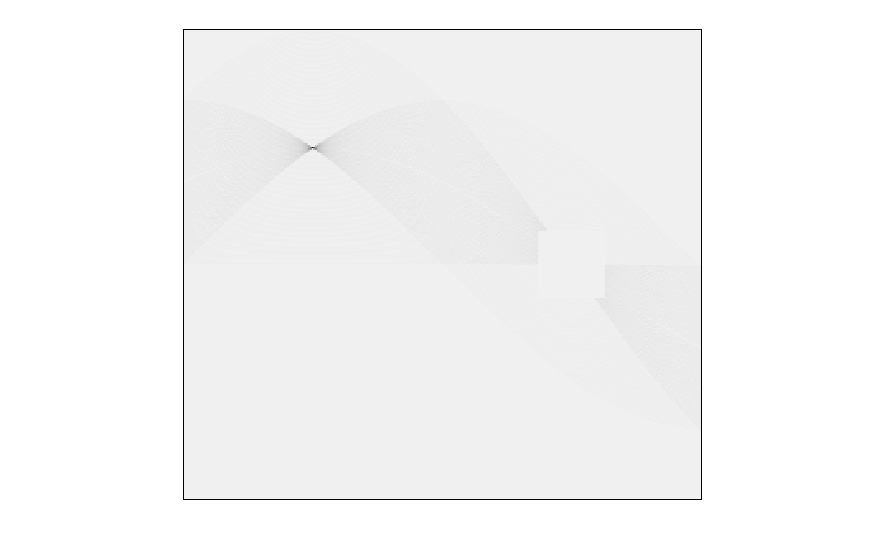
\includegraphics[width=0.82\textwidth]{images/ACCUM_NMS.png}
%		\caption{Аккумуляторный массив после применения NMS}
%	\end{figure}
%\end{frame}

\begin{frame}[shrink=5]{Преобразование Хафа: этапы работы}
	\textbf{Входные данные:} изображение после шумоподавления размера $m \times n$, шаги дискретизации $h_{\rho}, h_{\theta}$.

	\vspace{0.1cm}
	\textbf{Выходные данные:} оценки параметров найденных прямых $(\hat{\rho},\hat{\theta})$.

	\vspace{0.2cm}
	\begin{enumerate}
		\item Дискретизация пространства $(\rho,\theta)$ с шагами $h_\rho$ и $h_\theta$ и инициализация аккумулятора.
		\item Для каждой активной точки $(x,y)$ строится кривая $\rho(\theta)$ в пространстве параметров.
		\item Соответствующие ячейки аккумулятора получают голоса.
		\item По аккумулятору ищутся локальные максимумы, после чего оцениваются параметры прямых.
		\item По найденным $(\hat{\rho},\hat{\theta})$ восстанавливаются прямые на изображении.
	\end{enumerate}

	\vspace{0.2cm}
	\begin{block}{Важно}
		В текущей работе качество предобработки напрямую влияет на точность финальных оценок $\rho$ и $\theta$.
	\end{block}
\end{frame}

\section{Алгоритмы на основе CSSA}

\begin{frame}{Стандартные методы шумоподавления}
	\small
	\begin{itemize}
		\item В численном эксперименте алгоритм на основе \texttt{CSSA} сравнивается с методами \texttt{BM3D}, \texttt{Median}, \texttt{Wiener}, \texttt{Quantile 0.9}.
		\item \textbf{Median:} каждый пиксель заменяется медианой значений в локальном окне, что подавляет одиночные шумовые выбросы.
		\item \textbf{Wiener:} для каждого пикселя строится локальная линейная оценка по локальному среднему и локальной дисперсии.
		\item \textbf{BM3D:} похожие фрагменты изображения группируются, после чего выполняются преобразование, пороговая обработка и усреднение восстановленных блоков.
		\item \textbf{Quantile 0.9:} сохраняются только пиксели, значения которых не меньше 0.9-квантили яркости; остальные зануляются.
		\item Тем самым стандартные методы используют либо локальное сглаживание, либо нелокальное усреднение похожих фрагментов, либо пороговую обработку яркостей.
	\end{itemize}
\end{frame}

\begin{frame}{CSSA: вложение комплексного ряда}
	\small
	\begin{itemize}
		\item Рассматривается комплексный временной ряд
		\[
		z = (z_1,\dots,z_N).
		\]
		\item Цель метода CSSA --- представить ряд как сумму компоненты сигнала $\hat{\mathbf{S}} $ и шумовой компоненты $\hat{\mathbf{R}}$.
		\item Выбирается длина окна $L$, после чего задаётся $K = N - L + 1$.
		\item Оператор вложения переводит ряд в траекторную матрицу
		\[
		\mathbf{X} = \mathcal{T}_L(z) =
		\begin{pmatrix}
			z_1 & z_2 & \dots & z_K \\
			z_2 & z_3 & \dots & z_{K+1} \\
			\vdots & \vdots & \ddots & \vdots \\
			z_L & z_{L+1} & \dots & z_N
		\end{pmatrix}.
		\]
	\end{itemize}
\end{frame}

\begin{frame}{CSSA: SVD, группировка и восстановление}
	\small
	\begin{itemize}
		\item Для траекторной матрицы строится сингулярное разложение
		$\mathbf{X} = \sum_{i=1}^{d} \sqrt{\lambda_i}\,\mathbf{U}_i \mathbf{V}_i^{*}$.
		\item Компоненты, соответствующие сигналу, объединяются в группу $I$:
		$\mathbf{X}_{I} = \sum_{i\in I} \sqrt{\lambda_i}\,\mathbf{U}_i \mathbf{V}_i^{*}$.
		\item После диагонального усреднения получают оценку комплексного ряда
		$\widehat{z} = \mathcal{T}_L^{-1}\circ\mathcal{H}(\mathbf{X}_{I})$.
		\item Таким образом CSSA выступает как метод шумоподавления комплексного временного ряда.
	\end{itemize}

	\begin{block}{Применение в контексте шумоподавления изображений}
		Далее эта процедура используется внутри алгоритма \textbf{CSSA ROW-ROW}.
	\end{block}
\end{frame}

\begin{frame}{CSSA ROW-ROW: схема алгоритма}
	\small
	\textbf{Входные данные:} матрица изображения $\mathbf{M}\in\mathbb{R}^{m\times n}$
	и число сохраняемых компонент $k$.

	\textbf{Выходные данные:} оценка изображения $\widehat{\mathbf{S}}\in\mathbb{R}^{m\times n}$.

	\vspace{0.2cm}
	\textbf{Схема работы:}
	\begin{enumerate}
		\item Для каждой строки $\mathbf{m}^{(p)}$ вычисляется ДПФ:
		$\boldsymbol{\xi}^{(p)} = \mathcal{F}\bigl(\mathbf{m}^{(p)}\bigr)$, $p=1,\dots,m$.
		\item К каждому комплексному ряду $\boldsymbol{\xi}^{(p)}$ применяется CSSA.
		\item В разложении сохраняются $k$ компонент, после чего строится оценка ряда $\widehat{\boldsymbol{\xi}}^{(p)}$.
		\item По каждой строке выполняется обратное ПФ:
		$\widehat{\mathbf{s}}^{(p)} = \operatorname{Re}\!\Bigl(\mathcal{F}^{-1}\bigl(\widehat{\boldsymbol{\xi}}^{(p)}\bigr)\Bigr)$.
		\item Из строк $\widehat{\mathbf{s}}^{(1)},\dots,\widehat{\mathbf{s}}^{(m)}$ составляется матрица $\widehat{\mathbf{S}}$.
	\end{enumerate}
\end{frame}

\begin{frame}{Мотивировка алгоритма CSSA ROW-ROW}
	\small
	\begin{itemize}
		\item Для строки с одной яркой точкой имеем
		$\mathbf{x} = c\,\mathbf{e}_j + \boldsymbol{\varepsilon}$,
		где $\mathbf{e}_j$ --- базисный вектор, а $\boldsymbol{\varepsilon}$ --- гауссов шум.
		\item После преобразования Фурье
		$\mathcal{F}(\mathbf{x}) = c\,\boldsymbol{\omega}_j + \widetilde{\boldsymbol{\varepsilon}}$,
		где $\boldsymbol{\omega}_j=\mathcal{F}(\mathbf{e}_j)$ --- вектор комплексных экспонент, а
		$\widetilde{\boldsymbol{\varepsilon}}$ остаётся гауссовым вектором.
		\item Если
		$\mathbf{x} = \sum_{r=1}^{k} c_r \mathbf{e}_{j_r} + \boldsymbol{\varepsilon}$,
		то в частотной области получаем сумму $k$ комплексных векторов $c_r\boldsymbol{\omega}_{j_r}$ и гауссова шума.
		\item Сумма небольшого числа экспонент порождает низкоранговую траекторную матрицу, поэтому в CSSA естественно сохранять $k$ компонент.
	\end{itemize}
\end{frame}

\begin{frame}{CSSA ROW-ROW: пример}
	\begin{figure}
		\centering
		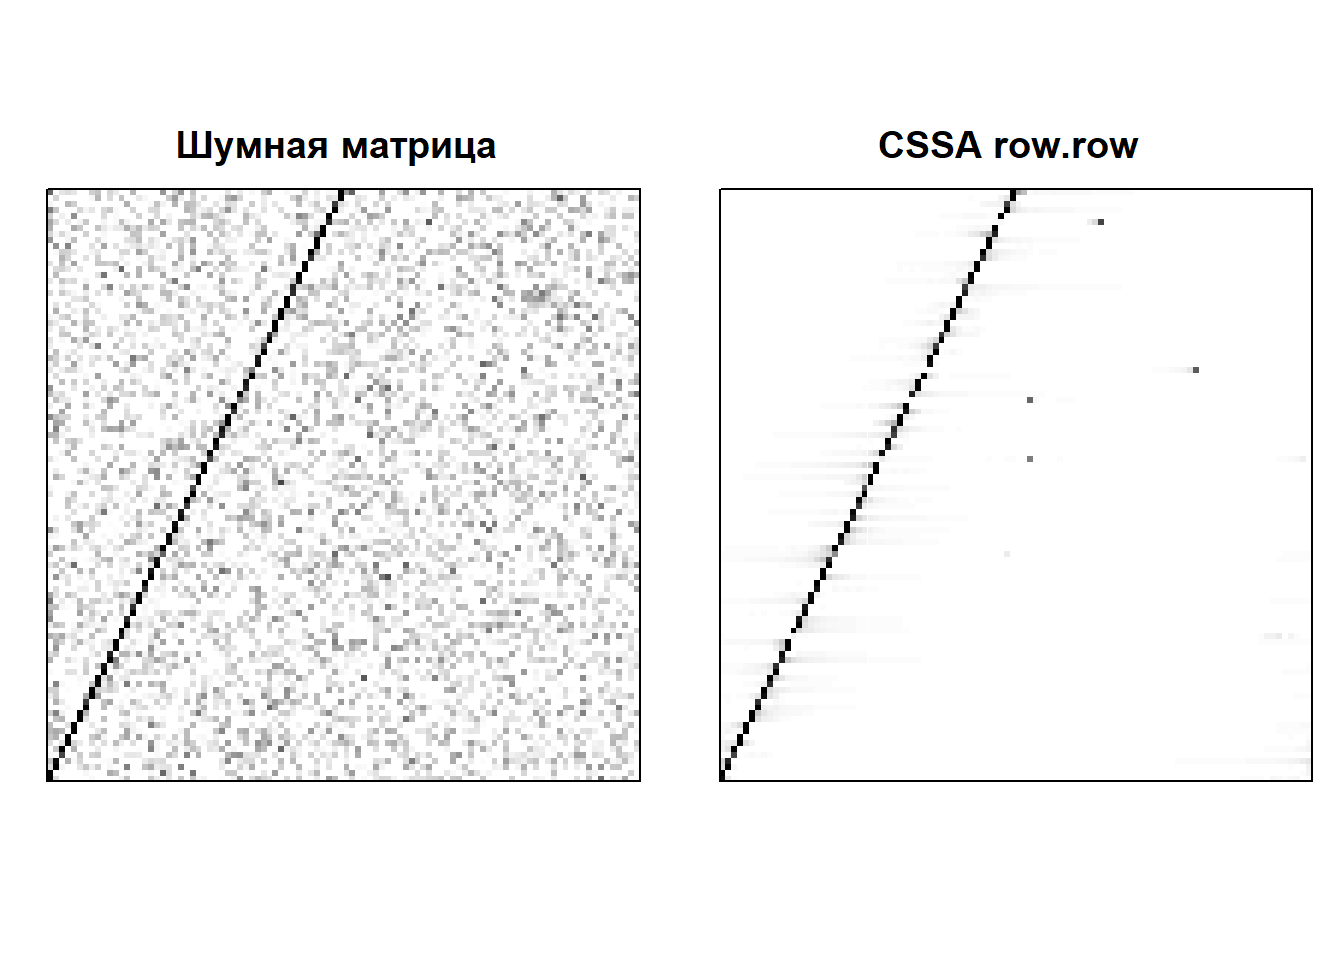
\includegraphics[width=0.8\textwidth]{images/demo-cssa-row-row-1.png}
		\caption{\parbox[t]{0.88\linewidth}{\centering Шумоподавление методом CSSA ROW-ROW, $n=m=100$, $\sigma=0.2$, прямая $y=2x-1$}}
	\end{figure}
\end{frame}

\section{Численное сравнение}

\begin{frame}{Схема численного эксперимента}
	\begin{itemize}
		\item Рассматривается изображение размера $100\times100$ с одной прямой.
		\item Уровень шума: $\sigma = 0.2$.
		\item Сравниваются методы шумоподавления \texttt{CSSA ROW-ROW}, \texttt{BM3D}, \texttt{Median}, \texttt{Wiener}, \texttt{Quantile 0.9}.
		\item После шумоподавления ко всем изображениям применяется один и тот же метод Хафа.
		\item Используются 4 конфигурации прямой и по 100 повторов на каждый метод.
	\end{itemize}
\end{frame}

\begin{frame}{Конфигурации прямых в эксперименте}
	\begin{figure}
		\centering
		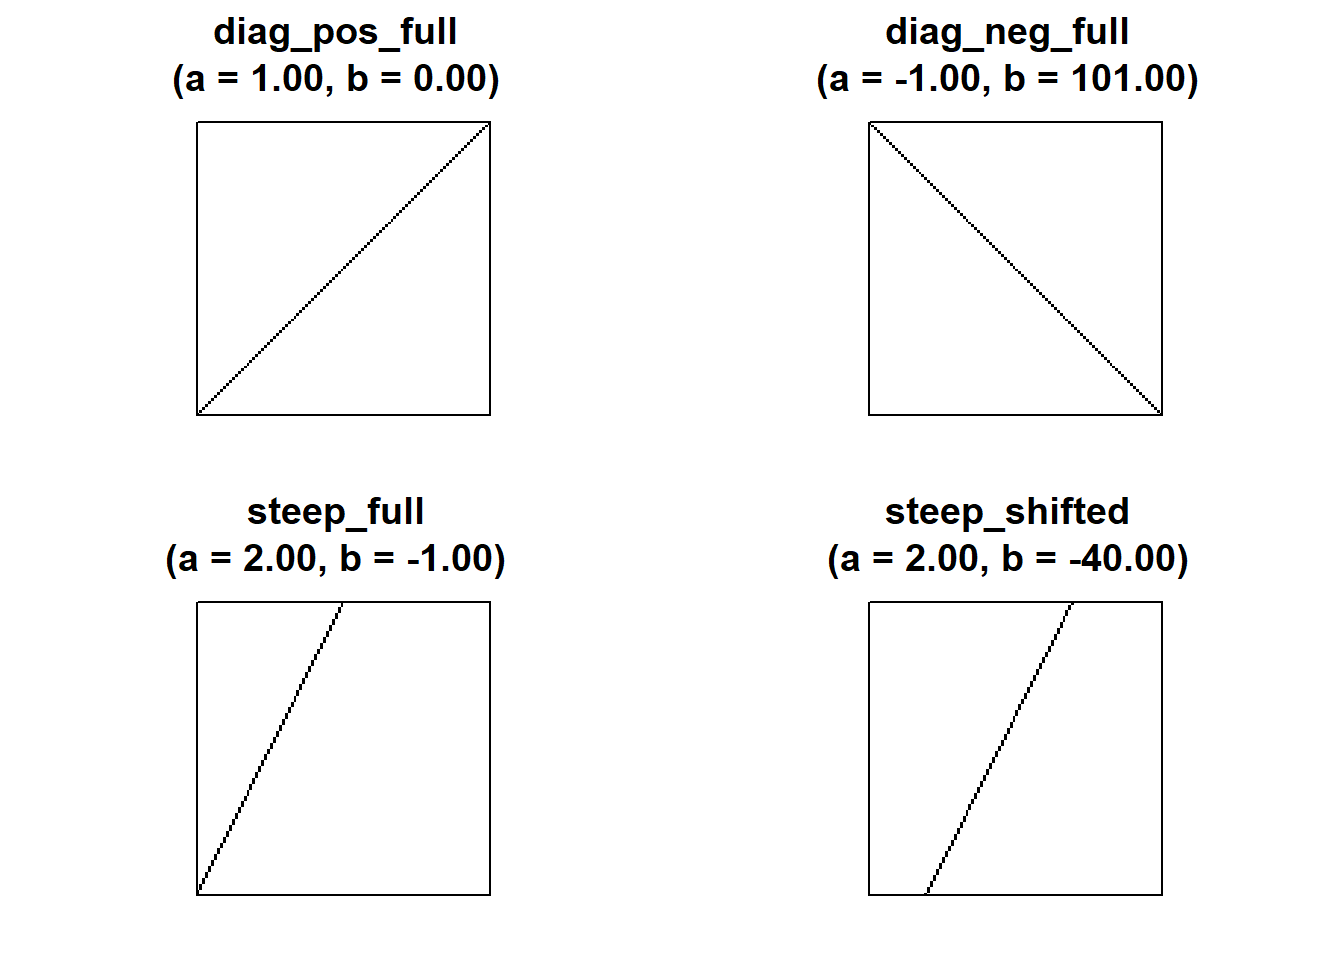
\includegraphics[width=0.84\textwidth]{images/configuration-preview-1.png}
		\caption{Конфигурации прямых, использованные в численном эксперименте}
	\end{figure}
\end{frame}

\begin{frame}{Покомпонентная метрика ошибки}
	\begin{itemize}
		\item В численном эксперименте параметры прямой оцениваются покомпонентно: отдельно по $\rho$ и отдельно по $\theta$.
		\item Для $N$ запусков рассчитываются
		\[
		\mathrm{MSE}_{\rho} = \frac{1}{N}\sum_{i=1}^{N}(\rho_i-\hat{\rho}_i)^2,
		\qquad
		\mathrm{MSE}_{\theta} = \frac{1}{N}\sum_{i=1}^{N}(\theta_i-\hat{\theta}_i)^2.
		\]
		\item Дополнительно для устойчивости к выбросам рассматривается медиана тех же покомпонентных квадратов ошибок.
	\end{itemize}
\end{frame}

\begin{frame}{Медианные ошибки параметров}
	\begin{table}[H]
		\centering
		\scriptsize
		\begin{tabular}{|l|c|c|}
			\hline
			Метод & median $\Delta_\rho$ & median $\Delta_\theta$ \\
			\hline
			CSSA ROW-ROW & \textbf{0.093483} & 0.0000178 \\
			BM3D & 0.200000 & 0.0000252 \\
			Median & 0.174544 & \textbf{0.0000145} \\
			Wiener & 160.100000 & 0.101089 \\
			Quantile 0.9 & \textbf{0.093483} & 0.0000178 \\
			\hline
		\end{tabular}
		\caption{Медианные покомпонентные ошибки по всем экспериментам}
	\end{table}

	\begin{block}{Парные сравнения лидеров}
		\scriptsize
		Для $\Delta_\rho$: \texttt{Quantile 0.9} vs \texttt{CSSA ROW-ROW}, критерий Вилкоксона,
		$p=4.7\cdot 10^{-14}$; предпочтителен \texttt{Quantile 0.9}.\\
		Для $\Delta_\theta$: \texttt{Median} vs \texttt{CSSA ROW-ROW}, критерий Вилкоксона,
		$p=1.9\cdot 10^{-17}$; предпочтителен \texttt{Median}.
	\end{block}
\end{frame}

\begin{frame}{Средние ошибки параметров}
	\begin{table}[H]
		\centering
		\scriptsize
		\begin{tabular}{|l|c|c|}
			\hline
			Метод & mean $\Delta_\rho$ & mean $\Delta_\theta$ \\
			\hline
			CSSA ROW-ROW & 457.535482 & 0.551325 \\
			BM3D & 192.197810 & 0.168978 \\
			Median & 42.030314 & 0.016628 \\
			Wiener & 1355.175000 & 0.664413 \\
			Quantile 0.9 & \textbf{0.096742} & \textbf{0.0000261} \\
			\hline
		\end{tabular}
		\caption{Средние покомпонентные ошибки по всем экспериментам}
	\end{table}

	\begin{block}{Парные сравнения лидеров}
		\scriptsize
		Для $\Delta_\rho$: \texttt{Quantile 0.9} vs \texttt{Median}, парный t-критерий,
		$p=0.052$; на уровне значимости $0.05$ различие не подтверждается.\\
		Для $\Delta_\theta$: \texttt{Quantile 0.9} vs \texttt{Median}, парный t-критерий,
		$p=0.0366$; предпочтителен \texttt{Quantile 0.9}.
	\end{block}
\end{frame}

%\begin{frame}[shrink=14]{Средние ошибки по $\rho$ для разных конфигураций}
%	\begin{table}[H]
%		\centering
%		\tiny
%		\begin{tabular}{|l|r|r|r|r|r|}
%			\hline
%			Конфигурация & CSSA ROW-ROW & BM3D & Median & Wiener & Quantile 0.9 \\
%			\hline
%			Положительная диагональ & 0.000000 & 2.330000 & 0.000000 & 0.000000 & 0.000000 \\
%			Отрицательная диагональ & 0.205786 & 74.432329 & 0.214007 & 5100.500000 & 0.174544 \\
%			Крутая прямая & 1829.923720 & 621.940948 & 101.940706 & 0.200000 & 0.200000 \\
%			Крутая смещённая & 0.012422 & 70.087964 & 65.966543 & 320.000000 & 0.012422 \\
%			\hline
%		\end{tabular}
%		\caption{Средние значения ошибки по параметру $\rho$ для разных конфигураций прямой}
%	\end{table}
%
%	\begin{block}{Парные сравнения лидеров}
%		\tiny
%		Положительная диагональ: \texttt{CSSA ROW-ROW} vs \texttt{Median}, $p=1.00$.\\
%		Отрицательная диагональ: \texttt{Quantile 0.9} vs \texttt{CSSA ROW-ROW}, $p=5.2\cdot 10^{-6}$; лучше \texttt{Quantile 0.9}.\\
%		Крутая прямая: \texttt{Quantile 0.9} vs \texttt{Wiener}, $p=1.00$.\\
%		Крутая смещённая: \texttt{CSSA ROW-ROW} vs \texttt{Quantile 0.9}, $p=1.00$.
%	\end{block}
%\end{frame}
%
%\begin{frame}[shrink=14]{Медианные ошибки по $\rho$ для разных конфигураций}
%	\begin{table}[H]
%		\centering
%		\tiny
%		\begin{tabular}{|l|r|r|r|r|r|}
%			\hline
%			Конфигурация & CSSA ROW-ROW & BM3D & Median & Wiener & Quantile 0.9 \\
%			\hline
%			Положительная диагональ & 0.000000 & 0.000000 & 0.000000 & 0.000000 & 0.000000 \\
%			Отрицательная диагональ & 0.174544 & 0.338974 & 0.174544 & 5100.500000 & 0.174544 \\
%			Крутая прямая & 12.622291 & 0.305573 & 0.305573 & 0.200000 & 0.200000 \\
%			Крутая смещённая & 0.012422 & 0.012422 & 0.012422 & 320.000000 & 0.012422 \\
%			\hline
%		\end{tabular}
%		\caption{Медианные значения ошибки по параметру $\rho$ для разных конфигураций прямой}
%	\end{table}
%
%	\begin{block}{Парные сравнения лидеров}
%		\tiny
%		Положительная диагональ: \texttt{CSSA ROW-ROW} vs \texttt{Median}, $p=1.00$.\\
%		Отрицательная диагональ: \texttt{Quantile 0.9} vs \texttt{CSSA ROW-ROW}, $p=1.3\cdot 10^{-5}$; лучше \texttt{Quantile 0.9}.\\
%		Крутая прямая: \texttt{Quantile 0.9} vs \texttt{Wiener}, $p=1.00$.\\
%		Крутая смещённая: \texttt{CSSA ROW-ROW} vs \texttt{Quantile 0.9}, $p=1.00$.
%	\end{block}
%\end{frame}
%
%\begin{frame}[shrink=14]{Средние ошибки по $\theta$ для разных конфигураций}
%	\begin{table}[H]
%		\centering
%		\tiny
%		\begin{tabular}{|l|r|r|r|r|r|}
%			\hline
%			Конфигурация & CSSA ROW-ROW & BM3D & Median & Wiener & Quantile 0.9 \\
%			\hline
%			Положительная диагональ & 0.000014 & 0.000064 & 0.000014 & 0.000014 & 0.000014 \\
%			Отрицательная диагональ & 0.000046 & 0.037483 & 0.000032 & 2.455460 & 0.000023 \\
%			Крутая прямая & 2.205234 & 0.386263 & 0.036016 & 0.101089 & 0.000063 \\
%			Крутая смещённая & 0.000004 & 0.252102 & 0.030450 & 0.101089 & 0.000004 \\
%			\hline
%		\end{tabular}
%		\caption{Средние значения ошибки по параметру $\theta$ для разных конфигураций прямой}
%	\end{table}
%
%	\begin{block}{Парные сравнения лидеров}
%		\tiny
%		Положительная диагональ: \texttt{CSSA ROW-ROW} vs \texttt{Median}, $p=1.00$.\\
%		Отрицательная диагональ: \texttt{Quantile 0.9} vs \texttt{Median}, $p=0.0213$; лучше \texttt{Quantile 0.9}.\\
%		Крутая прямая: \texttt{Quantile 0.9} vs \texttt{Median}, $p=0.125$; статистически значимых различий нет.\\
%		Крутая смещённая: \texttt{CSSA ROW-ROW} vs \texttt{Quantile 0.9}, $p=1.00$.
%	\end{block}
%\end{frame}
%
%\begin{frame}[shrink=14]{Медианные ошибки по $\theta$ для разных конфигураций}
%	\begin{table}[H]
%		\centering
%		\tiny
%		\begin{tabular}{|l|r|r|r|r|r|}
%			\hline
%			Конфигурация & CSSA ROW-ROW & BM3D & Median & Wiener & Quantile 0.9 \\
%			\hline
%			Положительная диагональ & 0.000014 & 0.000014 & 0.000014 & 0.000014 & 0.000014 \\
%			Отрицательная диагональ & 0.000021 & 0.000029 & 0.000021 & 2.455460 & 0.000021 \\
%			Крутая прямая & 3.974631 & 0.000145 & 0.000004 & 0.101089 & 0.000063 \\
%			Крутая смещённая & 0.000004 & 0.000004 & 0.000004 & 0.101089 & 0.000004 \\
%			\hline
%		\end{tabular}
%		\caption{Медианные значения ошибки по параметру $\theta$ для разных конфигураций прямой}
%	\end{table}
%
%	\begin{block}{Парные сравнения лидеров}
%		\tiny
%		Положительная диагональ: \texttt{CSSA ROW-ROW} vs \texttt{Median}, $p=1.00$.\\
%		Отрицательная диагональ: \texttt{Quantile 0.9} vs \texttt{Median}, $p=0.00189$; лучше \texttt{Quantile 0.9}.\\
%		Крутая прямая: \texttt{Median} vs \texttt{Quantile 0.9}, $p=1.3\cdot 10^{-8}$; лучше \texttt{Median}.\\
%		Крутая смещённая: \texttt{CSSA ROW-ROW} vs \texttt{Quantile 0.9}, $p=1.00$.
%	\end{block}
%\end{frame}

\begin{frame}{Итоги}
	\begin{itemize}
		\item Основное сравнение проводится покомпонентно: отдельно по $\rho$ и отдельно по $\theta$.
		\item По средним ошибкам лидирует \texttt{Quantile 0.9}; для $\Delta_\theta$ его преимущество над \texttt{Median} статистически значимо, а для $\Delta_\rho$ на уровне $0.05$ не подтверждается.
		\item По медианным ошибкам \texttt{Quantile 0.9} лучше \texttt{CSSA ROW-ROW} по $\rho$, а \texttt{Median} лучше \texttt{Quantile 0.9} по $\theta$.
		\item \texttt{CSSA ROW-ROW} остаётся рабочим методом шумоподавления, но в текущем эксперименте не является лучшим по итоговым парным сравнениям.
	\end{itemize}
\end{frame}

\begin{frame}{Список литературы}
	\begin{thebibliography}{99}
		\bibitem{book1} N.~Golyandina, V.~Nekrutkin, A.~Zhiglyavsky.
		\textit{Analysis of Time Series Structure: SSA and Related Techniques}.
		Chapman \& Hall/CRC, 2001.

		\bibitem{hough} R.O.~Duda, P.E.~Hart.
		\textit{Use of the Hough Transformation to Detect Lines and Curves in Pictures}.
		Communications of the ACM, 15(1):11--15, 1972.

		\bibitem{trickett} S.~R.~Trickett.
		\textit{F-xy eigenimage noise suppression}.
		Geophysics, 68(2):751--759, 2003.
	\end{thebibliography}
\end{frame}

\end{document}
